\section{Mercado de jogos}

A indústria de jogos eletrônicos está passando por um crescimento contínuo, impulsionada pelos avanços tecnológicos e pelas mudanças nas preferências dos consumidores. De acordo com um estudo conduzido pela empresa \textit{\gls{Newzoo}}, as projeções para o mercado global de jogos indicam um aumento aproximado de 3.4\% até o ano de 2025. Esse crescimento representa um potencial de lucro estimado em cerca de US\$ 211.2 bilhões em escala mundial, destacando o apelo universal dos jogos eletrônicos que ultrapassam barreiras culturais e geográficas, conforme ilustrado na Figura \ref{GlobalMarketForecast}.

A diversificação do público consumidor, incluindo crianças, adultos e idosos, tem gerado uma demanda crescente por uma variedade de jogos. Além disso, tendências como jogos \textit{\gls{Multiplayer}} online e jogos baseados em computação em nuvem, bem como avanços tecnológicos, como gráficos de alta qualidade, realidade virtual e dispositivos móveis poderosos, têm aumentado a acessibilidade aos jogos eletrônicos, contribuindo significativamente para a expansão do mercado.

\begin{figure}[H]
	\centering
	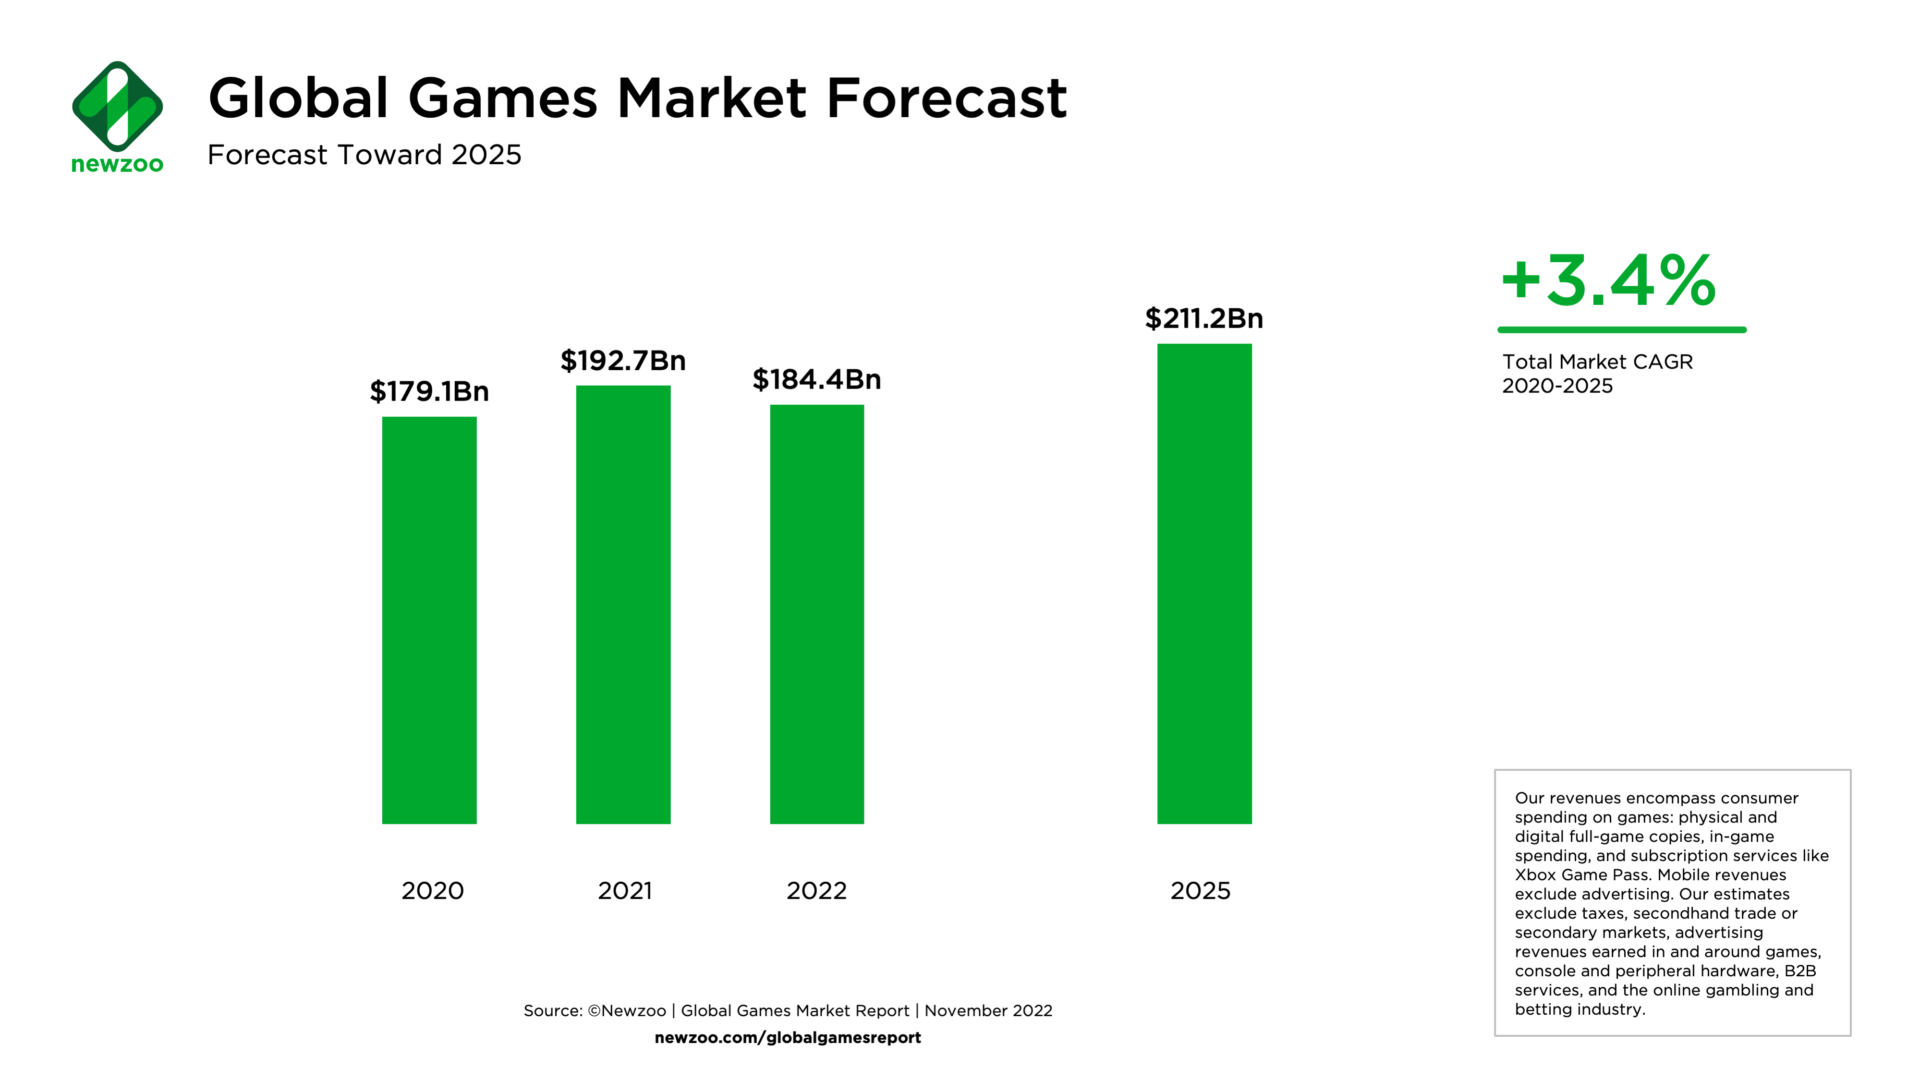
\includegraphics[scale=0.24]{imagens/revisaoLeitura/global_games_market_forecast.png}
	\caption{Global Market Forecast}
	\label{GlobalMarketForecast}
	\fonte{\cite{global_games_market}}
\end{figure}

Além de seu valor de entretenimento, a indústria de jogos eletrônicos possui impactos econômicos e sociais notáveis. O mercado de \textit{eSports} está crescendo exponencialmente, criando empregos para jogadores profissionais e profissionais relacionados. Socialmente, os jogos eletrônicos desempenham um papel crucial na formação de comunidades online, oferecendo um sentido de pertencimento e camaradagem em um mundo digitalizado.

O futuro da indústria de jogos eletrônicos é promissor, com a integração da inteligência artificial e tecnologias de aprendizado de máquina prometendo jogos mais dinâmicos e adaptativos. Além disso, a realidade aumentada está gerando experiências inovadoras que combinam o mundo físico e digital, indicando um caminho empolgante para a evolução dos jogos eletrônicos.

Para compreender plenamente a magnitude dessa cifra substancial, torna-se imperativo realizar uma comparação com setores de entretenimento mais consolidados, como a indústria cinematográfica e musical. Segundo dados da \textit{\gls{GrandViewResearch}}, esses setores alcançaram lucros na ordem de US\$ 90.1 bilhões, conforme evidenciado na Figura \ref{GlobalMoviesEntertainmentMarket}. A disparidade financeira entre os jogos eletrônicos e esses segmentos tradicionais ressalta a ascensão meteórica dos jogos na economia global, traçando um cenário claro e incontestável da crescente importância econômica dos videogames.

\begin{figure}[H]
	\centering
	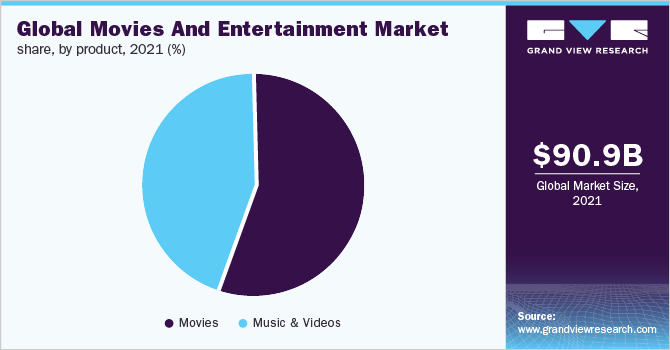
\includegraphics[scale=0.6]{imagens/revisaoLeitura/global_movies_entertainment_market.png}
	\caption{Global Movies Entertainment Market}
	\label{GlobalMoviesEntertainmentMarket}
	\fonte{\cite{global_films_musics_market}}
\end{figure}

A indústria cinematográfica, que já foi considerada um dos pilares fundamentais do entretenimento, agora enfrenta uma concorrência acirrada dos jogos eletrônicos. Esta transformação evidencia as preferências dos consumidores, e a capacidade dos jogos eletrônicos de se adaptarem às mudanças tecnológicas, oferecendo experiências interativas e imersivas que atraem públicos de todas as idades.

No campo da música, historicamente uma das formas de entretenimento mais lucrativas, os videogames também estão fazendo incursões significativas. A trilha sonora de jogos, muitas vezes composta por músicas originais e licenciadas, tornou-se uma parte integral da experiência de jogo. Além disso, eventos e competições de jogos eletrônicos frequentemente apresentam performances ao vivo de artistas musicais renomados, criando uma sinergia entre os dois mundos do entretenimento e ampliando ainda mais o alcance dos jogos eletrônicos. 

Nesse panorama, convém salientar que o êxito financeiro do mercado de jogos ultrapassa o resultado de um segmento isolado, consistindo, da complexa interação entre diversos setores dentro da indústria de jogos. A análise desses segmentos revela uma gama abrangente de possibilidades, incluindo Jogos de Computador, Consoles, Plataformas Móveis e Navegadores, todos contribuindo de maneiras distintas para a expansão contínua do mercado.

Um aspecto que merece destaque é a crescente importância dos jogos para dispositivos móveis nesse cenário multifacetado. Pesquisas recentes conduzidas pela renomada empresa \textit{\gls{Newzoo}} demonstram de forma clara que o setor de jogos para dispositivos móveis está destinado a liderar essa expansão. A Figura \ref{GlobalMarketPerSegment}, que corrobora essas descobertas, revela uma tendência ascendente notável nesse segmento específico da indústria de jogos.

\begin{figure}[H]
	\centering
	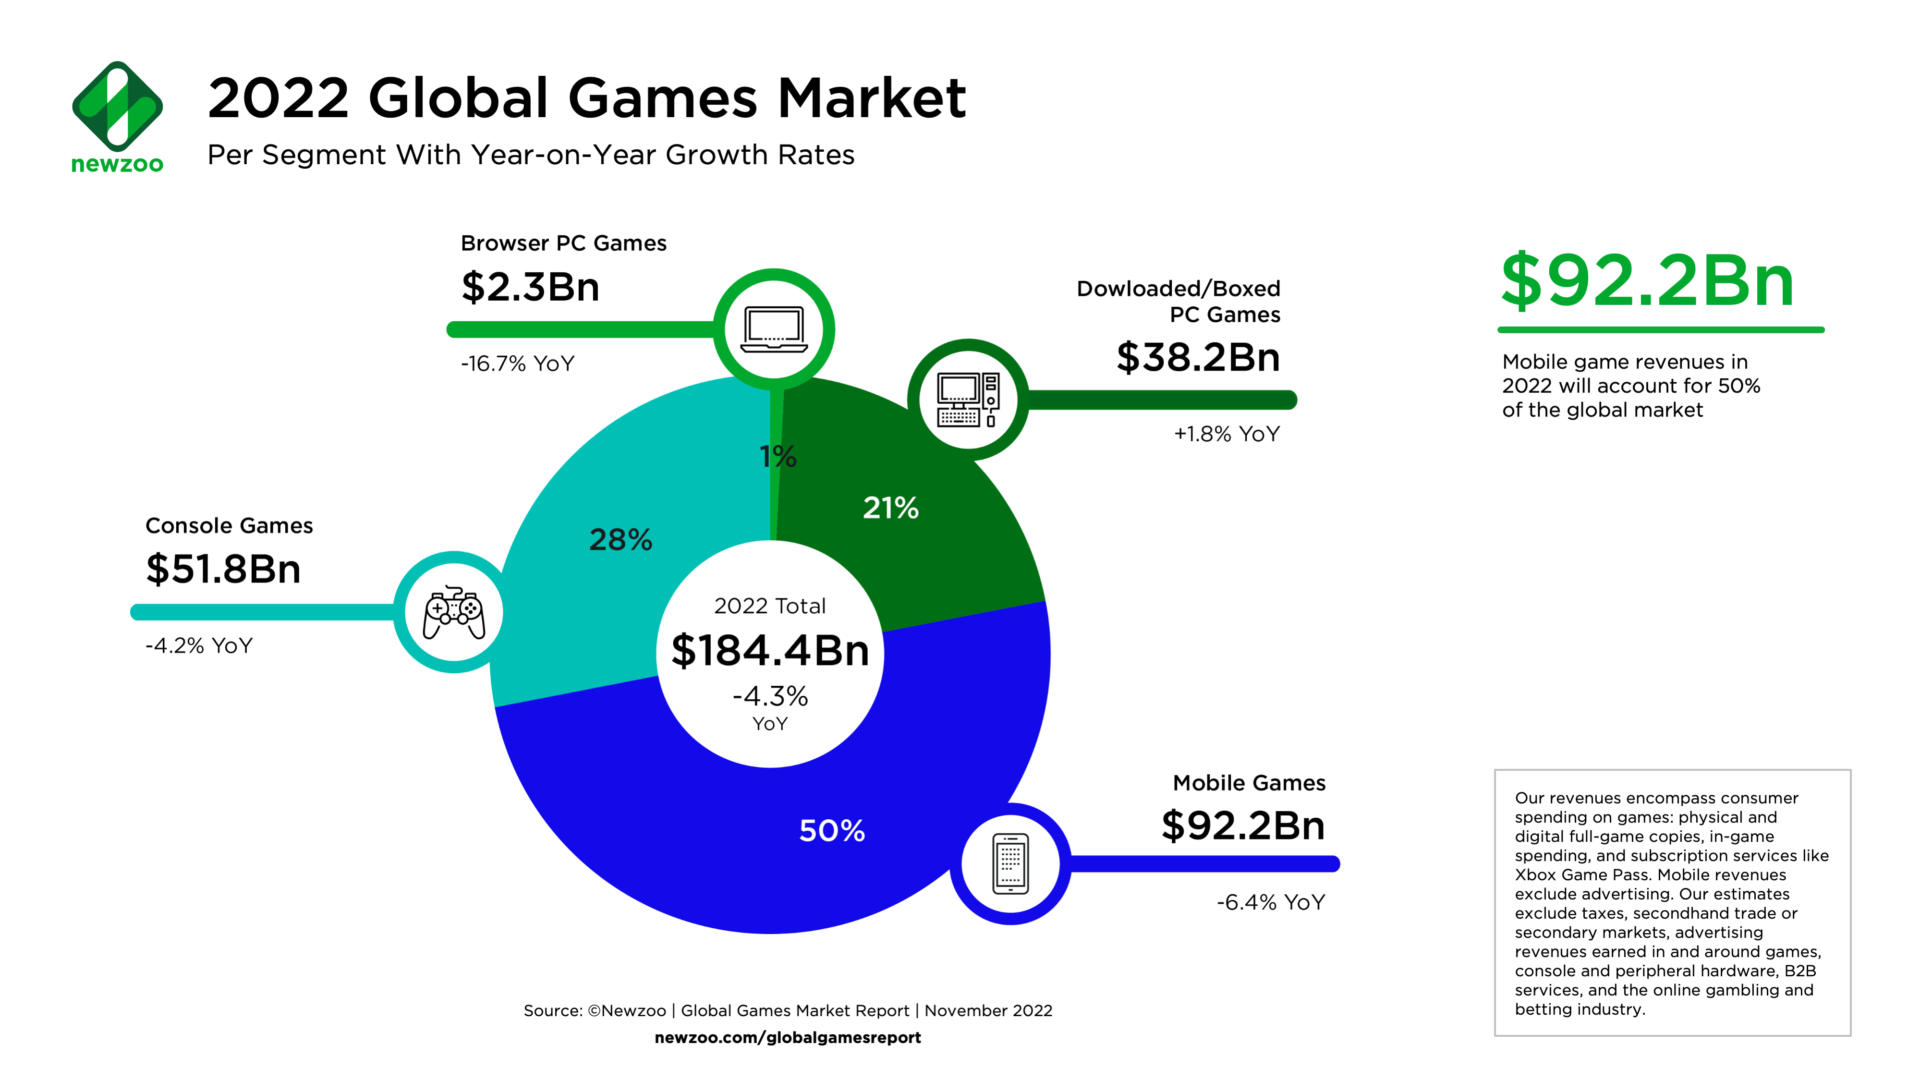
\includegraphics[scale=0.22]{imagens/revisaoLeitura/global_games_market_per_segment.png}
	\caption{Global Market Per Segment}
	\label{GlobalMarketPerSegment}
	\fonte{\cite{global_games_market}}
\end{figure}

A relevância desse crescimento exponencial no mercado de jogos móveis é inegável. Não apenas os dispositivos móveis estão cada vez mais acessíveis, mas também oferecem uma plataforma altamente conveniente para os jogadores, que podem desfrutar de uma variedade de jogos com apenas alguns toques na tela de seus \textit{smartphones} ou \textit{tablets}. Essa acessibilidade instantânea atrai os jogadores casuais, e cativa uma base de jogadores mais dedicada e ávida por experiências de alta qualidade.

Além disso, é fundamental notar que a diversificação de plataformas facilita o acesso aos jogos, e impulsiona a inovação na indústria. Desenvolvedores de jogos agora têm a oportunidade de explorar novas tecnologias e ideias em diferentes plataformas, levando a uma riqueza de opções para os consumidores. Essa competição saudável entre os segmentos da indústria de jogos resulta em uma ampla gama de produtos, desde jogos independentes inovadores até títulos \textit{\gls{AAA}} de grande orçamento, todos contribuindo para a riqueza e diversidade do mercado.